\chapter{Materials \& Methods}

% 학위 논문의 결과를 도출하는 데에 사용한 실험 재료와 방법을 타인이 반복 실험 시 동일한 결과를 얻을 수 있을 정도로 자세히 기술한다. 방법에 따라 다음과 같이 부제를 넣어 기술한다.f

% 예)
% 2.1 식물 재료 및 생장 조건
% 2.2 뿌리 관속 조직 관찰
% 2.3 유전자 발현 분석

\section{Space Optimization}

The core idea of \texttt{Petasearch} is actually sacrificing space for fast computation. However, the resources are not limitless. Thus, we would like to keep the cost of space as low as possible while keeping the searching speed high. In this section, we will discuss the space optimization techniques utilized to improve \texttt{Petasearch} prototype.

\subsection{Diff-index Compression} \label{section:diff-index_compression}

As is described in chapter 2, the diff-index created in the k-mer extraction step will store multiple \texttt{USHRT\_MAX} as long as the difference is larger than \texttt{USHRT\_MAX}. This will make any k-mer difference larger than $4 \times \mathtt{USHRT\_MAX} = 262140$ require a larger space to store than the original \texttt{unsigned long} representation. This situation is not uncommon especially when $k$ is large.

Also, in the prototypical implementation, the ID of the source sequence will also be stored multiple times in the ID table. This redundancy is both unnecessary and troublesome. It will increase the size of \texttt{Petasearch} data structures even more than the repeated \texttt{USHRT\_MAX} since the IDs are stored as \texttt{unsigned long} (64-bit integers).


\autoref{fig:k11_space} showed the space consumption of the diff-index created in the k-mer extraction step when $k = 11$. Without optimization, the diff-index (k-mer table) and its corresponding ID table will take up 17 GB of space for a merely 1GB-sized database.

To optimize the size of the diff-index, we devised the bit-squeezing technique to compress the difference between two adjacent k-mers:
For any 64-bit k-mer difference, we continuously fetch 15 bits into a write buffer starting from the least significant bits. We stop the retrieval until we encounter a zero chunk (15 bits of zeros).

To enable the correct decoding of the diff-index during the next phase, the sign bit of the last element in th write is set to \texttt{1} to indicate the end of encoding. Afterwards, we write all the elements in the write buffer to the diff-index. An example encoding process for differecne of value $2039432531946$ is shown in \autoref{fig:bit_squeeze_technique}. For ID table, the optimization is simple: we store the ID of the source sequence only once instead of repeatedly.

Using the bit-squeezing method, it is possible to obtain a maximum of five chunks, making the final space consumption larger than the size of a \texttt{unsigned long} integer. However, such situation only happens when the difference is larger than $\texttt{1UL << 59} = 576460752303423488$, which is extremely rare.

While decoding the compressed diff-index in the process of double-index search, we will reverse the bit-squeezing process through repeatedly retrieving 15 bits from the diff-index table until we encounter the chunk with the sign bit set to \texttt{1}. The decoded difference value will be add to the current k-mer. Moreover, since we do not store redundant IDs, the ID pointer will not be incremented until the end of k-mer decoding. \cref{algorithm:decode_kmer} showed the simplified pseudocode for k-mer decoding.


\begin{figpage}
  \begin{figure}
    \centering
    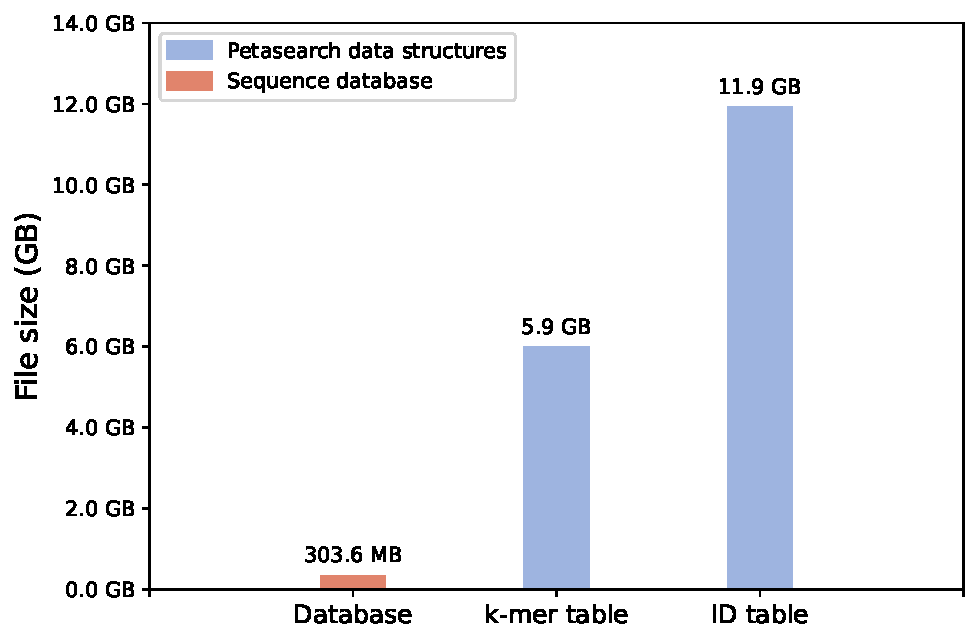
\includegraphics[width=.8\textwidth]{images/k11_space_consumption.pdf}
    \captionof{figure}{Visualizaiton of k-mer table and ID table sizes when $k = 11$. The database is the \texttt{UniProtKB/Swiss-Prot} database obtained through \texttt{mmseqs databases UniProtKB/Swiss-Prot swissprot tmp} command. Without optimization, the sizes of \texttt{petasearch} data structures are 6.46 times and 12.92 times larger than the sequence database.}
    \label{fig:k11_space}
  \end{figure}
  \begin{figure}
    \centering
    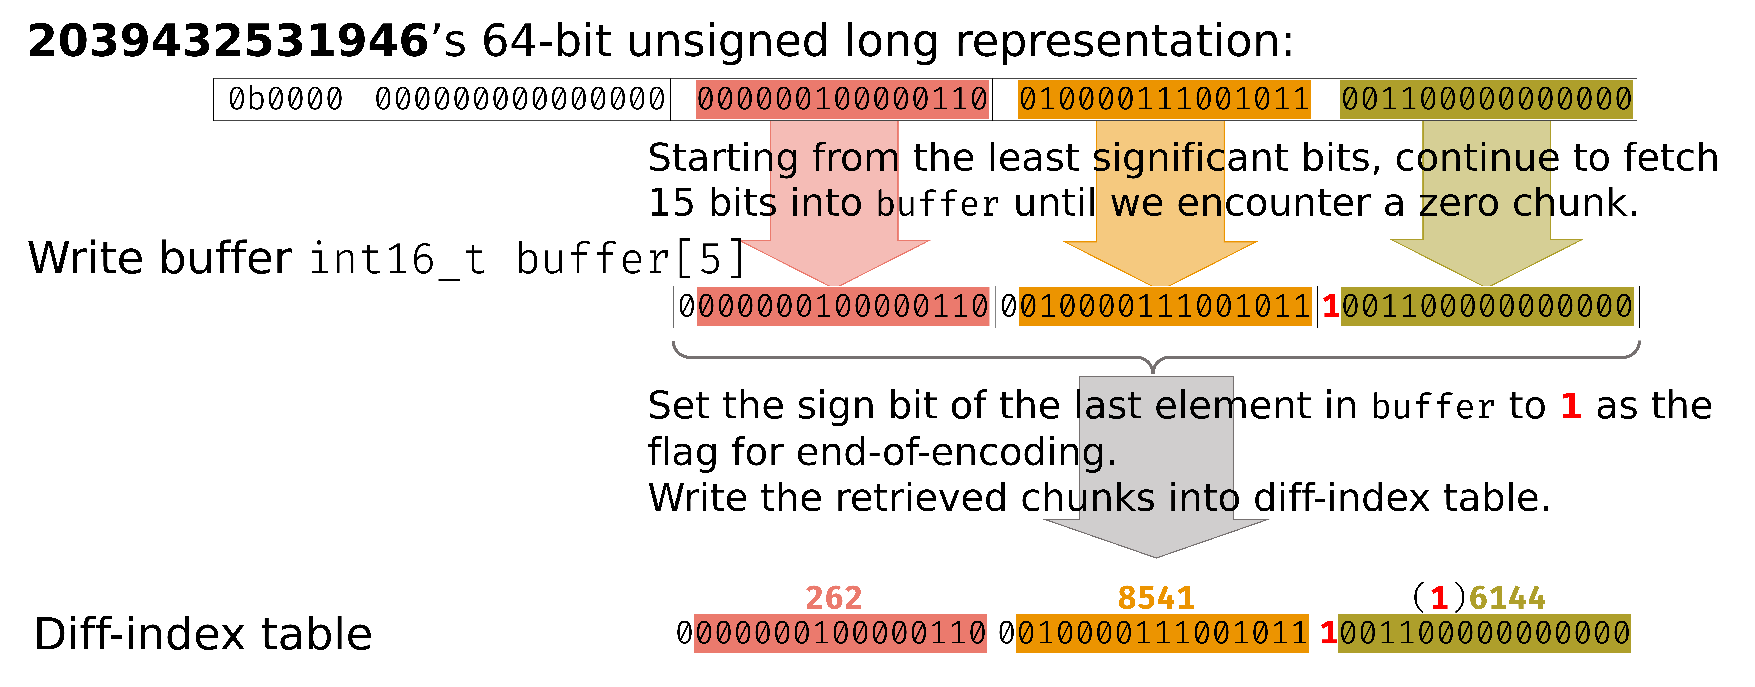
\includegraphics[width=\textwidth]{images/bit_squeezing_technique.pdf}
    \captionof{figure}{The example decoding process of difference index $2039432531946$. We first retrieve 15-bit chunks starting from the least significant bits and store them into a write buffer in the reverse order until we encounter a zero chunk. For $2039432531946$, its highest non-zero bit is $39$, which means that we need three 16-bit \texttt{short} to store it.}
    \label{fig:bit_squeeze_technique}
  \end{figure}
\end{figpage}

\begin{algorithm}[htbp]
  \begin{algorithmic}
    \Procedure{DecodeKmer}{$currentKmer$, $currentTargetKmerPtr$, $currentTargetIDPtr$}

    \State $currentDiffIndex \gets 0$\;
    % \State $X \gets x$
    % \State$ $N \gets n$
    \While{$*currentTargetKmerPtr > 0 $}\Comment{This means the sign bit is not 1. }
    \State $currentDiffIndex \gets\ \textsc{Get15Bits}(*currTargetKmerPtr)$
    \State $currentDiffIndex \gets currentDiffIndex \texttt{ << } 15$
    \State $\textsc{Next}(currTargetKmerPtr)$
    \EndWhile
    \State $currentDiffIndex \gets\ \textsc{Get15Bits}(*currTargetKmerPtr)$
    \State $currentKmer \gets currentKmer + currentDiffIndex$
    \State $\textsc{Next}(currTargetKmerPtr)$
    \State $currentTargetIDPtr \gets\ \textsc{Next}(currentTargetIDPtr)$
    \Return $currentKmer$
    \EndProcedure
    \caption{ Pseudocode for the k-mer decoding process} \label{algorithm:decode_kmer}
  \end{algorithmic}
\end{algorithm}

\subsection{Protein Sequence Compression}

For terabyte-size databases, the sequences themselves are also space consuming. To further reduce the size of the databases, we developed the \texttt{ASCII}-sqeezing technique.

Protein sequences are represented by a limited subset of \texttt{ASCII} characters, which are encoded by a single byte. However, as is shown in \autoref{fig:ascii_prot}, we only need 5 bits to represent all the amino acids. Therefore, we can squeeze every three amino acids into one 16-bit \texttt{short}. Similar to the bit-squeezing technique described in \cref{section:diff-index_compression}, we also use the sign bit to indicated the end of the compressed protein sequence. \autoref{fig:prot_seq_compress} showed an example compression process for glutathione (GSH).

The \texttt{ASCII}-squeezing technique is expected to produce a sqeuence database about $85\%$ of the original size.

\section{Speed Optimization}

Speed is the first and foremost concern of \texttt{Petasearch}. The speed of \texttt{Petaserch} prototype is already fast, but did not make it stand out too much from its competitors. In this section, we will introduce several techniques to further boost the speed of \texttt{Petasearch}.

\subsection{IO Performance Optimization}

\subsection{Fast third party libraries}


\begin{figpage}
  \begin{figure}
    \centering
    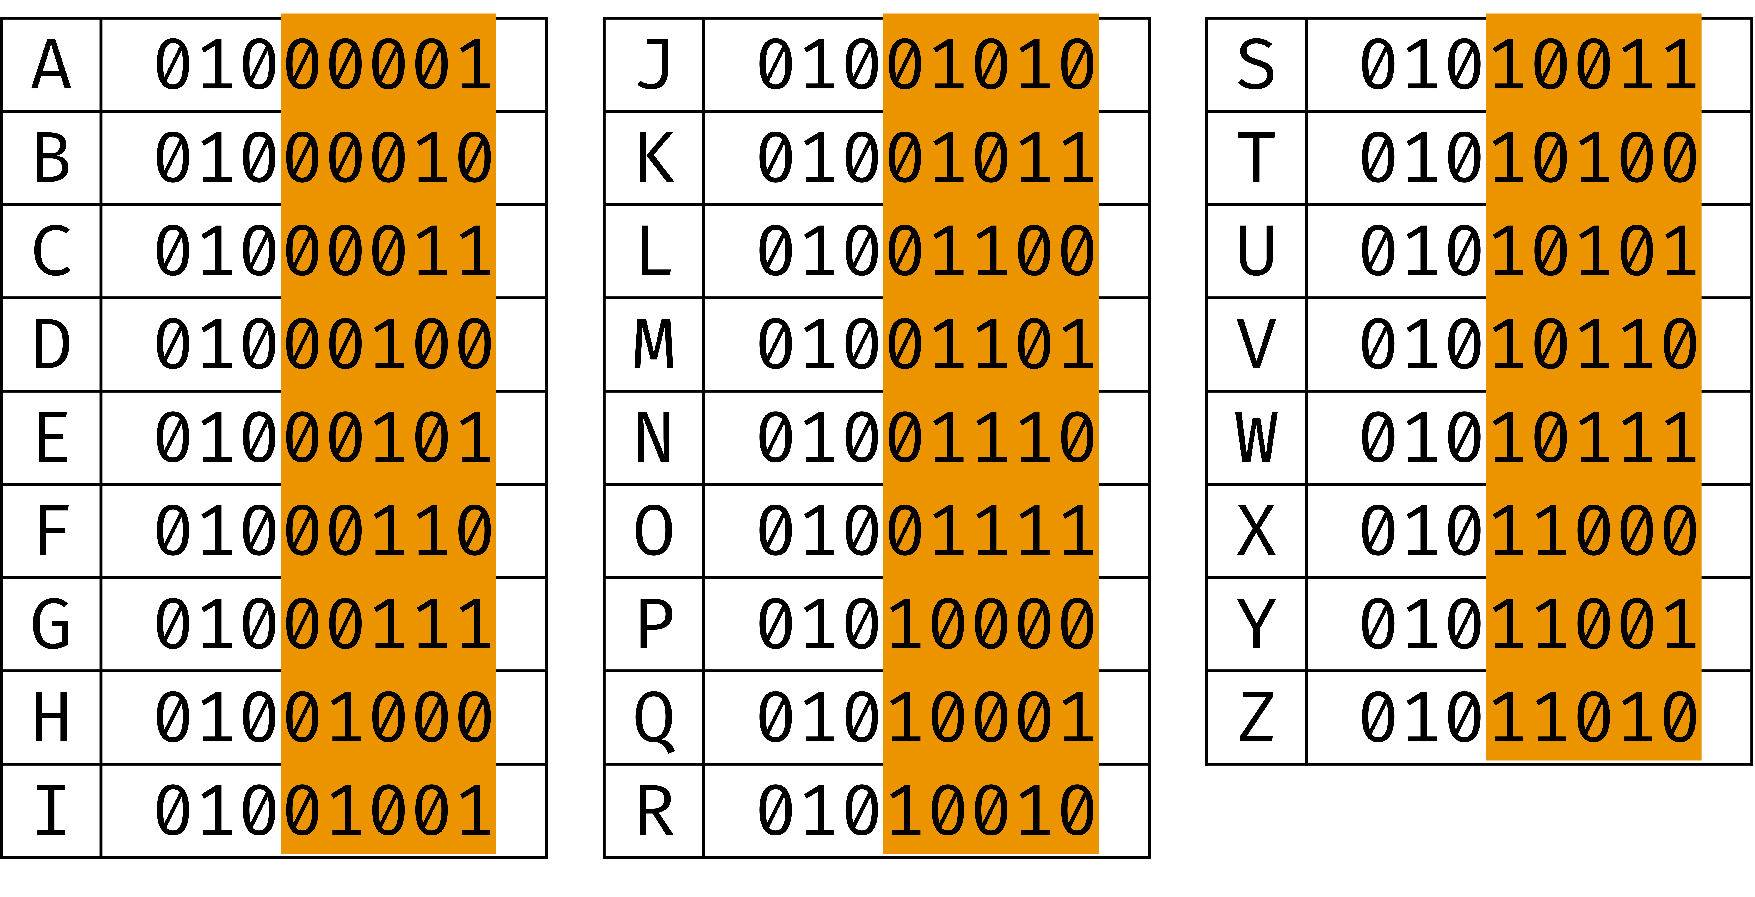
\includegraphics[width=.7\textwidth]{images/ASCII_prot.pdf}
    \caption{Part of the ASCII table, showing the bit representation of \texttt{A} to \texttt{Z} with the last 5 bits highlighted. It can be clearly seen that for \texttt{A} to \texttt{Z} in the English alphabet, we can represent them using only 5 bits instead of a whole byte (8 bits).}
    \label{fig:ascii_prot}
  \end{figure}
  \begin{figure}
    \centering
    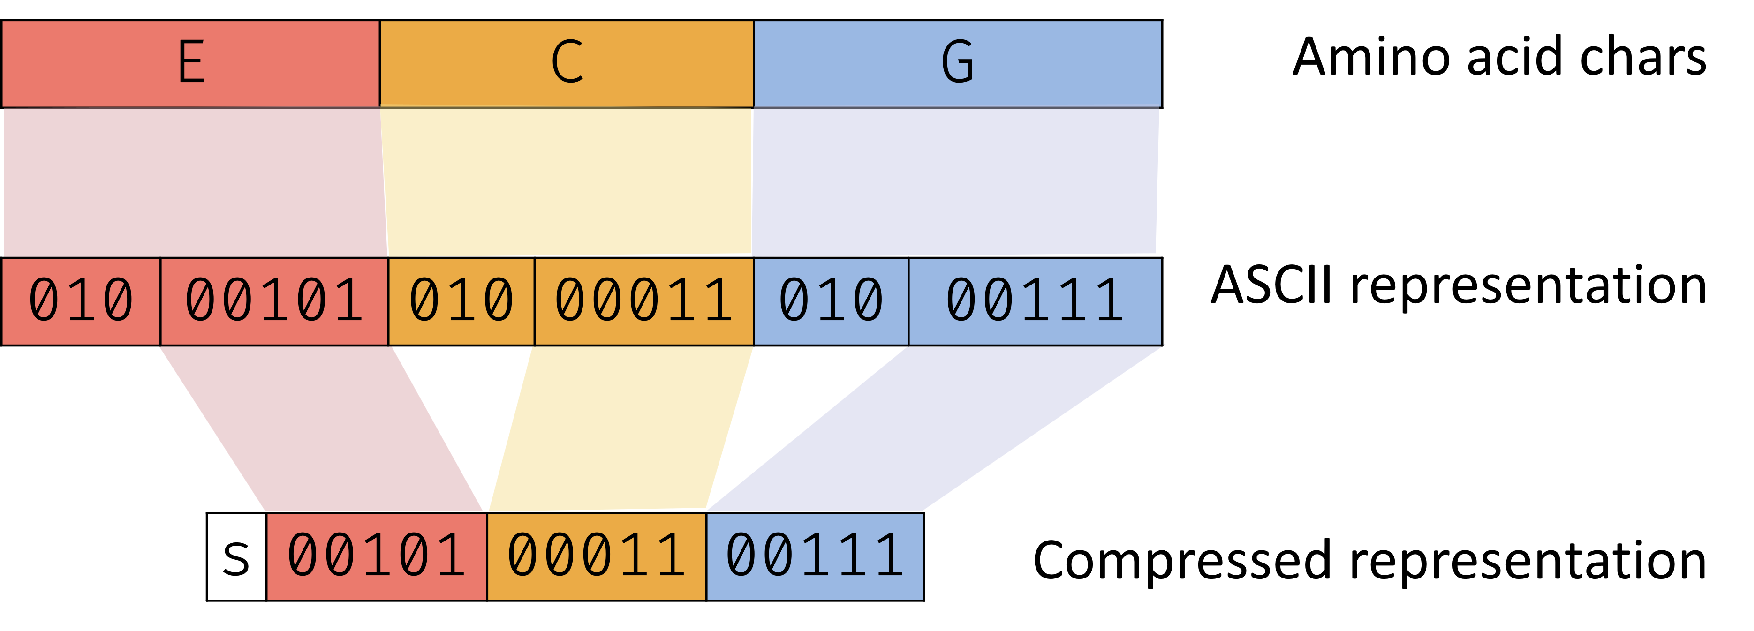
\includegraphics[width=\textwidth]{images/prot_seq_compress.pdf}
  \caption{The example compression of short peptide glutathione (GSH). GSH consists of only three amino acids: glutamate (E), cysteine (C), and glycine (G). We simply fetch the least significant 5 bits of each amino acid \texttt{char} and store them into a single 16-bit \texttt{short}.}
  \label{fig:prot_seq_compress}
\end{figure}
\end{figpage}

\section{Sensitivity Improvement}
